%%%%%%%%%%%%%%%%%%%%%%%%%%%%%%%%%%%%%%%%%%%%%%%%%%%%%%%%%%%%%%%%%%%%%%%%%%%%%%%%%%
\begin{frame}[fragile]\frametitle{}
\begin{center}
{\Large Multi Agents}
\end{center}
\end{frame}


%%%%%%%%%%%%%%%%%%%%%%%%%%%%%%%%%%%%%%%%%%%%%%%%%%%%%%%%%%%
\begin{frame}[fragile]\frametitle{Avoid Overloaded Agents}
    \begin{itemize}
        \item Don't overload a single AI agent with many MCP servers
        \item Leads to performance bottlenecks and poor scalability
        \item Use multiple agents for effective orchestration
    \end{itemize}
	
{\tiny (Ref: LinkedIn post by Rakesh Gohel)}
	
\end{frame}

%%%%%%%%%%%%%%%%%%%%%%%%%%%%%%%%%%%%%%%%%%%%%%%%%%%%%%%%%%%
\begin{frame}[fragile]\frametitle{Agents}
	
	\begin{center}
	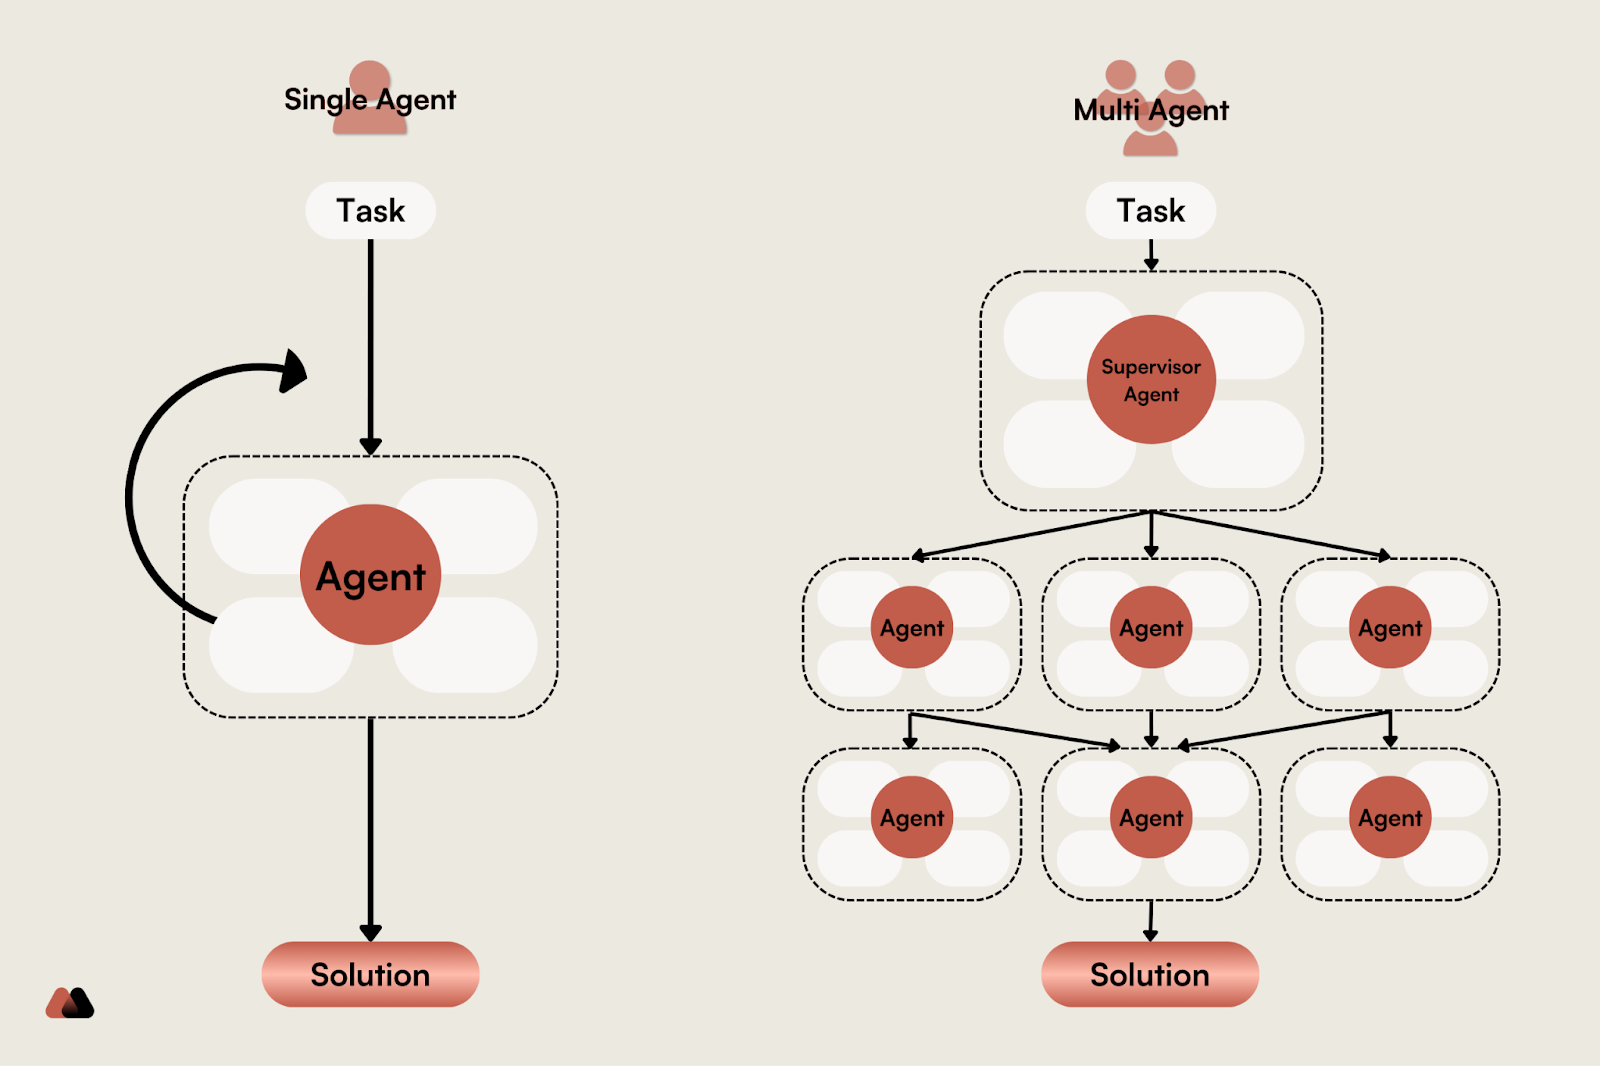
\includegraphics[width=0.8\linewidth,keepaspectratio]{agents1}
	\end{center}
	
{\tiny (Ref: Meet Agentic AI: The Vanguard of Modern Enterprise - Multimodal)}

\end{frame}


%%%%%%%%%%%%%%%%%%%%%%%%%%%%%%%%%%%%%%%%%%%%%%%%%%%%%%%%%%%
\begin{frame}[fragile]\frametitle{Why Multi-Agent Systems?}
    \begin{itemize}
        \item Specialised agents enable scalable automation
        \item Collaboration improves decision-making
        \item Parallel agents deliver faster results
        \item Real-time adaptation to dynamic inputs
    \end{itemize}
\end{frame}

%%%%%%%%%%%%%%%%%%%%%%%%%%%%%%%%%%%%%%%%%%%%%%%%%%%%%%%%%%%
\begin{frame}[fragile]\frametitle{Benefits of Multi-Agent Workflow}
    \begin{itemize}
        \item Single-agent systems are limited in scalability
        \item Multi-agent systems are modular and efficient
        \item Better for solving complex, dynamic problems
        \item Mimics real-world team collaboration
    \end{itemize}
\end{frame}

%%%%%%%%%%%%%%%%%%%%%%%%%%%%%%%%%%%%%%%%%%%%%%%%%%%%%%%%%%%
\begin{frame}[fragile]\frametitle{Popular Multi-Agent Patterns}
    \begin{itemize}
        \item Choose design patterns based on task needs
        \item Six effective patterns streamline development
        \item Supports better orchestration and coordination
    \end{itemize}
\end{frame}

%%%%%%%%%%%%%%%%%%%%%%%%%%%%%%%%%%%%%%%%%%%%%%%%%%%%%%%%%%%
\begin{frame}[fragile]\frametitle{Multi-Agent Patterns}
	
	\begin{center}
	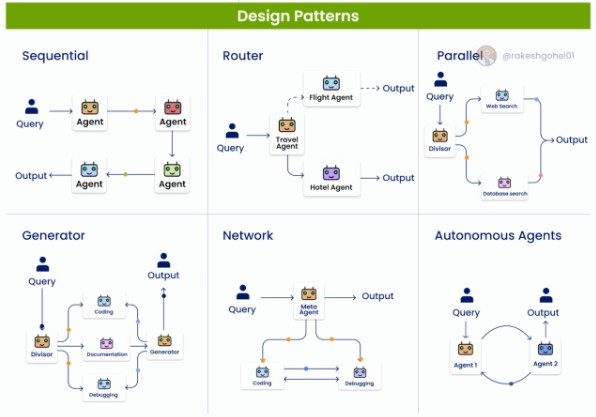
\includegraphics[width=0.8\linewidth,keepaspectratio]{agents2}
	\end{center}
	
{\tiny (Ref: LinkedIn post by Rakesh Gohel)}

\end{frame}


%%%%%%%%%%%%%%%%%%%%%%%%%%%%%%%%%%%%%%%%%%%%%%%%%%%%%%%%%%%
\begin{frame}[fragile]\frametitle{1. Sequential Pattern}
    \begin{itemize}
        \item Agents execute one after another in a chain
        \item Each refines or transforms the output
        \item Use cases: ETL pipelines, Q\&A verification
    \end{itemize}
\end{frame}

%%%%%%%%%%%%%%%%%%%%%%%%%%%%%%%%%%%%%%%%%%%%%%%%%%%%%%%%%%%
\begin{frame}[fragile]\frametitle{2. Router Pattern}
    \begin{itemize}
        \item Central router delegates tasks to specialists
        \item Acts like an API gateway
        \item Use cases: Customer support, service orchestration
    \end{itemize}
\end{frame}

%%%%%%%%%%%%%%%%%%%%%%%%%%%%%%%%%%%%%%%%%%%%%%%%%%%%%%%%%%%
\begin{frame}[fragile]\frametitle{3. Parallel Pattern}
    \begin{itemize}
        \item Divides tasks into independent parallel subtasks
        \item Aggregates results after parallel processing
        \item Use cases: Info retrieval, financial risk analysis
    \end{itemize}
\end{frame}

%%%%%%%%%%%%%%%%%%%%%%%%%%%%%%%%%%%%%%%%%%%%%%%%%%%%%%%%%%%
\begin{frame}[fragile]\frametitle{4. Generator Pattern}
    \begin{itemize}
        \item Iterative loop: divisor → specialists → generator → feedback
        \item Enables draft-refine workflows
        \item Use cases: Code generation, design documentation
    \end{itemize}
\end{frame}

%%%%%%%%%%%%%%%%%%%%%%%%%%%%%%%%%%%%%%%%%%%%%%%%%%%%%%%%%%%
\begin{frame}[fragile]\frametitle{5. Network Pattern}
    \begin{itemize}
        \item Fully meshed agents with bidirectional links
        \item Overseen by a central meta-agent
        \item Use cases: Design, security, compliance reviews
    \end{itemize}
\end{frame}

%%%%%%%%%%%%%%%%%%%%%%%%%%%%%%%%%%%%%%%%%%%%%%%%%%%%%%%%%%%
\begin{frame}[fragile]\frametitle{6. Autonomous Agents Pattern}
    \begin{itemize}
        \item Agents operate in decentralised, looped interactions
        \item No central coordinator needed
        \item Use cases: Embodied agents, autonomous navigation
    \end{itemize}
\end{frame}

%%%%%%%%%%%%%%%%%%%%%%%%%%%%%%%%%%%%%%%%%%%%%%%%%%%%%%%%%%%%%%%%%%%%%%%%%%%%%%%%%%
\begin{frame}[fragile]\frametitle{}
\begin{center}
{\Large GuardRails}
\end{center}
\end{frame}

%%%%%%%%%%%%%%%%%%%%%%%%%%%%%%%%%%%%%%%%%%%%%%%%%%%%%%%%%%%
\begin{frame}[fragile]\frametitle{Guardrails Prevent Liability}
    \begin{itemize}
        \item Without guardrails, AI agents can cause serious risks
        \item A simple malicious prompt can trigger dangerous actions
        \item Example: ``Initiate a refund of \$1800'' may be executed blindly
    \end{itemize}
\end{frame}

%%%%%%%%%%%%%%%%%%%%%%%%%%%%%%%%%%%%%%%%%%%%%%%%%%%%%%%%%%%
\begin{frame}[fragile]\frametitle{GuardRails}
	
	\begin{center}
	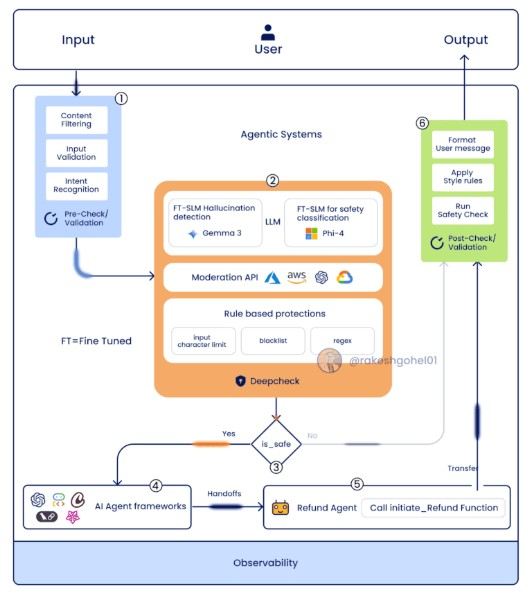
\includegraphics[width=0.8\linewidth,keepaspectratio]{agents3}
	\end{center}
	
{\tiny (Ref: LinkedIn post by Rakesh Gohel)}

\end{frame}


%%%%%%%%%%%%%%%%%%%%%%%%%%%%%%%%%%%%%%%%%%%%%%%%%%%%%%%%%%%
\begin{frame}[fragile]\frametitle{How Guardrails Help}
    \begin{itemize}
        \item Guardrails detect, filter, and block unsafe inputs
        \item Protect agent workflows from abuse and mistakes
        \item Ensure system behaves safely and predictably
    \end{itemize}
\end{frame}

%%%%%%%%%%%%%%%%%%%%%%%%%%%%%%%%%%%%%%%%%%%%%%%%%%%%%%%%%%%
\begin{frame}[fragile]\frametitle{1. Pre-Check \& Validation}
    \begin{itemize}
        \item Filters inputs before reaching the AI model
        \item Includes content filtering and intent detection
        \item Flags malicious, nonsensical, or off-topic prompts
        \item First line of defense in any AI pipeline
    \end{itemize}
\end{frame}

%%%%%%%%%%%%%%%%%%%%%%%%%%%%%%%%%%%%%%%%%%%%%%%%%%%%%%%%%%%
\begin{frame}[fragile]\frametitle{2. Agentic Guardrails}
    \begin{itemize}
        \item Safety logic embedded inside the agent system
        \item Uses fine-tuned small LMs and strict rules
        \item Helps prevent unsafe actions from within
    \end{itemize}
\end{frame}

%%%%%%%%%%%%%%%%%%%%%%%%%%%%%%%%%%%%%%%%%%%%%%%%%%%%%%%%%%%
\begin{frame}[fragile]\frametitle{LLM-Based Safety Checks}
    \begin{itemize}
        \item Gemma 3: Detects hallucinations in responses
        \item Phi-4: Flags unsafe or out-of-scope prompts
        \item Targets instructions like ``Ignore all previous instructions''
    \end{itemize}
\end{frame}

%%%%%%%%%%%%%%%%%%%%%%%%%%%%%%%%%%%%%%%%%%%%%%%%%%%%%%%%%%%
\begin{frame}[fragile]\frametitle{Moderation APIs}
    \begin{itemize}
        \item Use APIs from OpenAI, AWS, Azure, etc.
        \item Catch toxicity, PII, and policy violations
        \item Adds an additional moderation layer to the pipeline
    \end{itemize}
\end{frame}

%%%%%%%%%%%%%%%%%%%%%%%%%%%%%%%%%%%%%%%%%%%%%%%%%%%%%%%%%%%
\begin{frame}[fragile]\frametitle{Rule-Based Protections}
    \begin{itemize}
        \item Blacklists block known prompt injection phrases
        \item Regex filters catch dangerous patterns
        \item Input length limits prevent oversized payloads
    \end{itemize}
\end{frame}

%%%%%%%%%%%%%%%%%%%%%%%%%%%%%%%%%%%%%%%%%%%%%%%%%%%%%%%%%%%
\begin{frame}[fragile]\frametitle{3. Deepcheck Safety Validation}
    \begin{itemize}
        \item Central logic gate: \texttt{is\_safe}
        \item Routes safe prompts to AI agents
        \item Unsafe prompts are diverted to fallback agents
    \end{itemize}
\end{frame}

%%%%%%%%%%%%%%%%%%%%%%%%%%%%%%%%%%%%%%%%%%%%%%%%%%%%%%%%%%%
\begin{frame}[fragile]\frametitle{4. AI Agent Frameworks \& Handoffs}
    \begin{itemize}
        \item Once validated, input goes to correct agent
        \item Example: Refund Agent handles refund logic
        \item Ensures only safe instructions reach execution layer
    \end{itemize}
\end{frame}

%%%%%%%%%%%%%%%%%%%%%%%%%%%%%%%%%%%%%%%%%%%%%%%%%%%%%%%%%%%
\begin{frame}[fragile]\frametitle{5. Refund Agent Execution}
    \begin{itemize}
        \item Final agent in the chain performs the task
        \item Secure function call handles the refund logic
        \item Operates only after multilayer validation
    \end{itemize}
\end{frame}

%%%%%%%%%%%%%%%%%%%%%%%%%%%%%%%%%%%%%%%%%%%%%%%%%%%%%%%%%%%
\begin{frame}[fragile]\frametitle{6. Post-Check \& Output Validation}
    \begin{itemize}
        \item Output reviewed before being sent to user
        \item Checks formatting, style, and safety again
        \item Prevents accidental disclosure or unsafe responses
    \end{itemize}
\end{frame}

%%%%%%%%%%%%%%%%%%%%%%%%%%%%%%%%%%%%%%%%%%%%%%%%%%%%%%%%%%%
\begin{frame}[fragile]\frametitle{Observability Layer}
    \begin{itemize}
        \item Logs every step: input → logic → output
        \item Enables auditing, debugging, and improvement
        \item Critical for maintaining trust in AI systems
    \end{itemize}
\end{frame}

%%%%%%%%%%%%%%%%%%%%%%%%%%%%%%%%%%%%%%%%%%%%%%%%%%%%%%%%%%%
\begin{frame}[fragile]\frametitle{Key Takeaways}
    \begin{itemize}
        \item AI agents need more than good models
        \item Guardrails ensure safety, traceability, and fallbacks
        \item Systems thinking is essential for reliable automation
    \end{itemize}
\end{frame}

%%%%%%%%%%%%%%%%%%%%%%%%%%%%%%%%%%%%%%%%%%%%%%%%%%%%%%%%%%%%%%%%%%%%%%%%%%%%%%%%%%
\begin{frame}[fragile]\frametitle{}
\begin{center}
{\Large Agentic RAG}
\end{center}
\end{frame}

%%%%%%%%%%%%%%%%%%%%%%%%%%%%%%%%%%%%%%%%%%%%%%%%%%%%%%%%%%%
\begin{frame}[fragile]\frametitle{Agentic RAG: RAG is Here to Stay}
    \begin{itemize}
        \item Agentic RAG proves the lasting value of RAG systems
        \item Used by Glean AI, Perplexity, Harvey, and others
        \item Ideal for complex enterprise workflows
    \end{itemize}
\end{frame}

%%%%%%%%%%%%%%%%%%%%%%%%%%%%%%%%%%%%%%%%%%%%%%%%%%%%%%%%%%%
\begin{frame}[fragile]\frametitle{Comparison}
	
	\begin{center}
	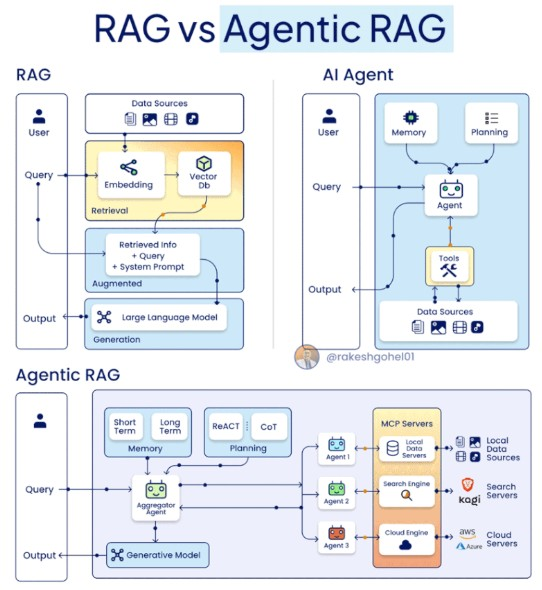
\includegraphics[width=0.8\linewidth,keepaspectratio]{agents4}
	\end{center}
	
{\tiny (Ref: LinkedIn post by Rakesh Gohel)}

\end{frame}


%%%%%%%%%%%%%%%%%%%%%%%%%%%%%%%%%%%%%%%%%%%%%%%%%%%%%%%%%%%
\begin{frame}[fragile]\frametitle{What is RAG (Retrieval Augmented Generation)?}
    \begin{itemize}
        \item Combines external data retrieval with LLM generation
        \item Ensures grounded and up-to-date responses
        \item Enhances reliability and relevance of output
    \end{itemize}
\end{frame}

%%%%%%%%%%%%%%%%%%%%%%%%%%%%%%%%%%%%%%%%%%%%%%%%%%%%%%%%%%%
\begin{frame}[fragile]\frametitle{RAG Workflow Overview}
    \begin{itemize}
        \item \textbf{1. Retrieval:} Query is embedded and relevant data is fetched from vector DB
        \item \textbf{2. Augmentation:} Retrieved data merged with query + system prompt
        \item \textbf{3. Generation:} LLM generates final response using augmented prompt
    \end{itemize}
\end{frame}

%%%%%%%%%%%%%%%%%%%%%%%%%%%%%%%%%%%%%%%%%%%%%%%%%%%%%%%%%%%
\begin{frame}[fragile]\frametitle{AI Agents in the Loop}
    \begin{itemize}
        \item Handle incoming queries and analyze intent
        \item Use memory and planning (ReACT, Reflexion)
        \item Fetch real-time data using tools and APIs
        \item Generate answers using reasoning and context
    \end{itemize}
\end{frame}

%%%%%%%%%%%%%%%%%%%%%%%%%%%%%%%%%%%%%%%%%%%%%%%%%%%%%%%%%%%
\begin{frame}[fragile]\frametitle{How Agentic RAG Combines RAG + Agents}
    \begin{itemize}
        \item Agents manage RAG's embedding and retrieval steps
        \item Dynamically choose data sources based on query
        \item Augment RAG prompts with planning and external tool data
        \item Deliver more precise and contextual outputs
    \end{itemize}
\end{frame}

%%%%%%%%%%%%%%%%%%%%%%%%%%%%%%%%%%%%%%%%%%%%%%%%%%%%%%%%%%%
\begin{frame}[fragile]\frametitle{Operational Workflow of Agentic RAG}
    \begin{itemize}
        \item \textbf{1. Query Routing:} Directs query to right agent
        \item \textbf{2. Context Retention:} Maintains short and long-term memory
        \item \textbf{3. Task Planning:} Chooses tools and retrieval plan
        \item \textbf{4. Data Fetching:} Retrieves from KBs using tools (e.g., vector search)
        \item \textbf{5. Prompt Optimisation:} Merges retrieved info + prompt + reasoning
        \item \textbf{6. Response Generation:} Final LLM output is generated and returned
    \end{itemize}
\end{frame}

%%%%%%%%%%%%%%%%%%%%%%%%%%%%%%%%%%%%%%%%%%%%%%%%%%%%%%%%%%%
\begin{frame}[fragile]\frametitle{Why Agentic RAG Matters}
    \begin{itemize}
        \item Enables smarter, more adaptive responses
        \item Combines memory, planning, retrieval, and reasoning
        \item Revolutionizing AI in enterprise applications
    \end{itemize}
\end{frame}


%%%%%%%%%%%%%%%%%%%%%%%%%%%%%%%%%%%%%%%%%%%%%%%%%%%%%%%%%%%%%%%%%%%%%%%%%%%%%%%%%%
\begin{frame}[fragile]\frametitle{}
\begin{center}
{\Large Claude Research Multi Agents}
\end{center}
\end{frame}

%%%%%%%%%%%%%%%%%%%%%%%%%%%%%%%%%%%%%%%%%%%%%%%%%%%%%%%%%%%
\begin{frame}[fragile]\frametitle{Claude Research: Multi-Agent Architecture}
    \begin{itemize}
        \item Anthropic shared insights into Claude's multi-agent architecture
        \item Real-world example of production-grade agent systems
        \item Highlights challenges, benefits, and practical design
    \end{itemize}
\end{frame}

%%%%%%%%%%%%%%%%%%%%%%%%%%%%%%%%%%%%%%%%%%%%%%%%%%%%%%%%%%%
\begin{frame}[fragile]\frametitle{Architecture}
	
	\begin{center}
	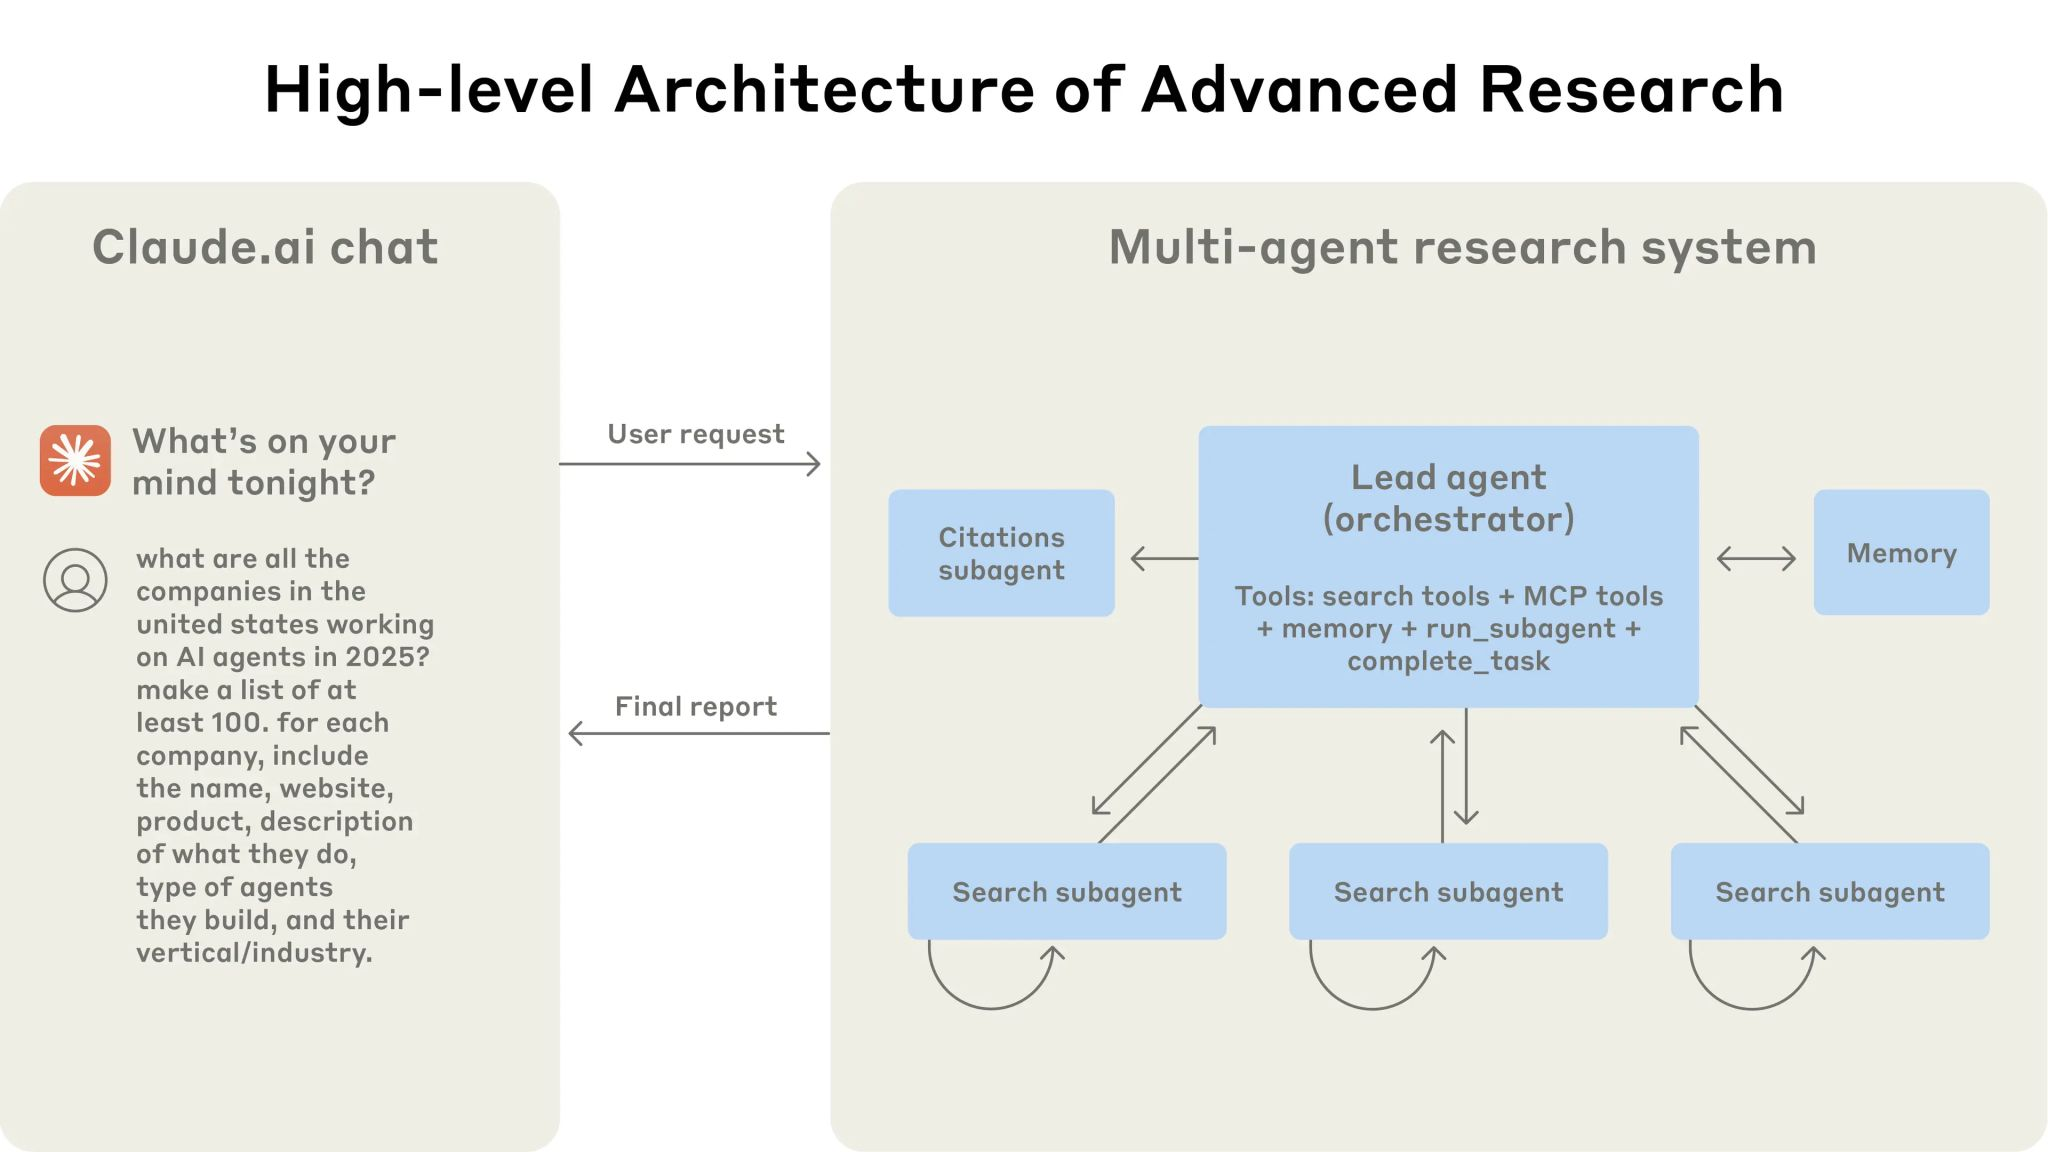
\includegraphics[width=0.8\linewidth,keepaspectratio]{agents5}
	\end{center}
	
{\tiny (Ref: LinkedIn post by Jerry Liu)}

\end{frame}

%%%%%%%%%%%%%%%%%%%%%%%%%%%%%%%%%%%%%%%%%%%%%%%%%%%%%%%%%%%
\begin{frame}[fragile]\frametitle{Not All Use Cases Need Multi-Agents}
    \begin{itemize}
        \item Some domains require shared context among agents
        \item High interdependencies reduce multi-agent effectiveness
        \item Not every task benefits from parallel agent workflows
    \end{itemize}
\end{frame}

%%%%%%%%%%%%%%%%%%%%%%%%%%%%%%%%%%%%%%%%%%%%%%%%%%%%%%%%%%%
\begin{frame}[fragile]\frametitle{Single vs Multi-Agent Debate}
    \begin{itemize}
        \item Similar point made by Cognition's ``Don't Build Multi-Agents''
        \item Both agree: multi-agents fit a specific class of problems
        \item Focus should be on identifying those right-fit use cases
    \end{itemize}
\end{frame}

%%%%%%%%%%%%%%%%%%%%%%%%%%%%%%%%%%%%%%%%%%%%%%%%%%%%%%%%%%%
\begin{frame}[fragile]\frametitle{Sub-Agents as Tools, Not Peers}
    \begin{itemize}
        \item Claude's system treats sub-agents like tools
        \item No explicit agent-to-agent handoffs
        \item Simplifies control and orchestration
    \end{itemize}
\end{frame}

%%%%%%%%%%%%%%%%%%%%%%%%%%%%%%%%%%%%%%%%%%%%%%%%%%%%%%%%%%%
\begin{frame}[fragile]\frametitle{Agents Improve Tool Interfaces}
    \begin{itemize}
        \item Claude uses a tool testing agent to refine tool descriptions
        \item Agent rewrites unclear interfaces after testing failures
        \item Result: 40\% reduction in task time for future agents
    \end{itemize}
\end{frame}

%%%%%%%%%%%%%%%%%%%%%%%%%%%%%%%%%%%%%%%%%%%%%%%%%%%%%%%%%%%
\begin{frame}[fragile]\frametitle{Self Improving Agents in Practice}
    \begin{itemize}
        \item Tool ergonomics improved through feedback loops
        \item Agents help reduce integration complexity
        \item Smarter interface   fewer downstream errors
    \end{itemize}
\end{frame}

%%%%%%%%%%%%%%%%%%%%%%%%%%%%%%%%%%%%%%%%%%%%%%%%%%%%%%%%%%%
\begin{frame}[fragile]\frametitle{Synchronous Execution   Bottlenecks}
    \begin{itemize}
        \item Claude's agents wait synchronously for sub agent results
        \item Simplifies coordination, but delays execution
        \item Creates sequential bottlenecks in agent chains
    \end{itemize}
\end{frame}

%%%%%%%%%%%%%%%%%%%%%%%%%%%%%%%%%%%%%%%%%%%%%%%%%%%%%%%%%%%
\begin{frame}[fragile]\frametitle{The Case for Async Architectures}
    \begin{itemize}
        \item Event driven models allow async agent execution
        \item Each agent acts as events arrive—faster coordination
        \item Matches design in frameworks like LlamaIndex workflows
    \end{itemize}
\end{frame}

%%%%%%%%%%%%%%%%%%%%%%%%%%%%%%%%%%%%%%%%%%%%%%%%%%%%%%%%%%%
\begin{frame}[fragile]\frametitle{Key Lessons from Claude Research}
    \begin{itemize}
        \item Use multi agent design selectively and purposefully
        \item Let agents optimize tools and interfaces over time
        \item Consider async architectures to eliminate bottlenecks
    \end{itemize}
\end{frame}
